\section{MapReduce, Apache Spark, GraphX}

In this section, we review the concept of MapReduce. Then we introduce the
in-memory MapReduce system, Apache Spark, and GraphX, the built-in graph
processing framework of Spark, on which InferSpark is built.

\subsection{MapReduce}

MapReduce is a widely-known simplistic programming model for parallelizing and
distributing computation on large datasets \sjtucite{dean04}. The model is
inspired by two functions in functional programming: the ``map'' function that
transforms each element in a set of data and the ``reduce'' function that
summarizes the data. A dataset is viewed as a collection of key-value pairs.
The user program has to supply two functions, ``map'' and ``reduce''. The
``map'' function takes a key-value pair as input and transforms it into a set
of intermediate key-value pairs. Then the intermediate key-value pairs are
grouped according to the keys. Finally, the ``reduce'' function is passed a
list of values and their common key in the grouped results and produce a
summary of the list.

\begin{figure}[t]
\centering
\includegraphics[width=0.9\linewidth,clip]{figs/mapreduce.eps}
\caption{MapReduce}
\label{fig:mapreduce}
\end{figure}

A typical MapReduce system (e.g. Apache Hadoop MapReduce) is shown in
\figref{fig:mapreduce}. There is a master that handles MapReduce job submitted
by user programs and schedules map/reduce tasks, $M$ mappers that perform the
map phase and $R$ reducers that perform the reduce phase. In the map phase, a
mapper reads the assigned splits of input and calls the ``map'' function on
each of the input key-value pair. It then writes the results into $R$ local
intermediate files. If the user program supplies an optional ``combiner''
function, the key-value pairs with the same key are combined by that function
before they are written to the intermediate files. The ``combiner'' function is
usually a partial ``reduce'' which reduces the size of data shuffle between the
map phase and the reduce phase. The intermediate files are shuffled to the
appropriate reducer, which then sorts the key-value pairs and calls the
``reduce'' function on the key-value pairs with the same key to produce the
outputs.

The whole process of a MapReduce job involves a lot of I/O with the underlying
storage and network. First the inputs are read either from local file systems
or distributed file systems. The intermediate files are written by the mappers
to the local disks. The reducers performs remote reads to get the intermediate
files to be shuffled to them. The reducers may need to sort the key-value
pairs in order to group the pairs with the same keys, where external sort may
be used if the pairs are too large to fit in the main memory. MapReduce is a
easy-to-use yet efficient framework for simple jobs like word count. It,
however, is not suitable for multi-stage pipelined jobs since output written out
from the last iteration has to be read from the file system in the next iteration 
as input. The I/O between pipelined MapReduce Jobs are essentially wasted
while the amount of time spent on that could be substantial for multi-stage
pipelined MapReduce jobs.


\subsection{Apache Spark}

Apache Spark \sjtucite{Zaharia:2010:SCC:1863103.1863113} solves the problem of
wasted I/O between MapReduce Jobs by storing the datasets in the main memory
whenever possible. The datasets are always in the memory except the case where
they are read from the file system for the first time or they have to be
shuffled across the cluster.

Spark represents datasets as Resilient Distributed Datasets (RDDs)
\sjtucite{Zaharia:2012:RDD:2228298.2228301}, which are immutable fault-tolerant
datasets distributed across the cluster. The ``map'' function is generalized
into {\tt transformations} such as ``map'', ``flatMap'', ``filter'' and the
``reduce'' function is generalized into {\tt actions} such as ``count'',
``reduce'', ``foreach''. Transformations are lazily applied and each
transformation creates a new immutable RDD.  Hence, multiple transformations
won't apply until an action is called on the final RDD. An action triggers a
Spark job. A job is further divided into stages between two of which there's
data shuffle. User program can also specify what RDDs to be cached or uncached
in the memory or disk to avoid re-computation.

\subsection{GraphX}

\begin{figure}[h]
	\centering
	\subfigure[Graph]{
		\label{fig:graphx_raw_graph}
		\includegraphics[width=0.2\linewidth,clip]{figs/graphx_raw_graph.eps}
	}
	\subfigure[RDDs]{
		\label{fig:graphx_graph_rep}
		\includegraphics[width=0.4\linewidth,clip]{figs/graphx_graph_rep.eps}
	}
	\subfigure[Triplet View]{
		\label{fig:graphx_triplet_view}
		\includegraphics[width=0.3\linewidth,clip]{figs/graphx_triplet_view.eps}
	}
	\caption{GraphX}
\end{figure}

GraphX \sjtucite{graphx} is the built-in graph processing framework on Spark.
It represents a graph as a VertexRDD and an EdgeRDD
(\figref{fig:graphx_graph_rep}), which stores vertices and edges as their names
suggest. The vertices and edges in GraphX are usually associated with
attributes. They are also stored in the VertexRDD and EdgeRDD. GraphX also lazily
maintains an edge triplet view, where an edge triplet is a 5-tuple of the two
ends of the edges along with all of their attributes.

GraphX adopts a vertex-cut approach to graph partitioning, as opposed to the
common edge-cut approach. It could partitions edges with the same source vertex
into different partitions in order to balance the load. Replica of referenced
vertices are lazily maintained in edge partitions to facilitate the edge
triplet view.  The shipment of vertices is essentially a distributed join
between VertexRDD and EdgeRDD.

GraphX mainly supports the Gather-Apply-Scatter (GAS) computation model, where
each vertex receives messages, updates itself and sends new messages to
neighbors. The famous Pregel \sjtucite{pregel} model is a special case of GAS where
only vertices that actually receive messages remain active in the next
iteration. The model can be implemented using two key APIs of GraphX:
``aggregateMessages'' and ``joinVertices''. The ``aggregateMessages'' API
takes a ``sendMsg'' function that is invoked on each active edge in the
specified direction. Then the messages to the same destination is merged using
the ``mergeFunc''. Finally, it generates a VertexRDD with
messages as attributes of the receivers. The ``joinVertices'' API can be used
to join the original vertices with the messages in order to update the
vertices.

GraphX maintains auxiliary data structures in the partitions to facilitate fast
joins and scans required by the above design. Each vertex partition contains a
routing table that specifies what vertices should be sent to what 
partitions. Each edge partition contains a clustered index on the source ID of
edges. When the proportion of active edges is smaller than a threshold and
whether an edge is active is related to the source ID, GraphX will prefer the
faster index scan to scanning all the edges.
